\section{What the sharp local theorem makes possible}
\label{sec:applications}

\subsection{A substantial reduction in the search endpoint}
The two bounds below have exactly the same fixed aggregate objective. In both, \(\rho\ge r_{h_0}\), the coefficients are integral, and the total Gauss budget is at most \(B\):
\[
 H_{\mathrm{old}}=h_0+\ceil{p^{h_0}B(h_0+B+2)},
 \qquad
 H_*=h_0+\floor{p^{h_0-1}B}.
\]
The first was sufficient; the second is optimal uniformly over the permitted coefficients. Examples computed with exact arithmetic are:
\begin{center}
\begin{tabular}{@{}rrrrr@{}}
\toprule
\(p\)&\(h_0\)&\(B\)&Previous endpoint&Sharp endpoint\\
\midrule
2&1&1&9&2\\
2&1&10&261&11\\
3&2&1&47&5\\
3&2&5&407&17\\
2&3&10&1203&43\\
5&2&2&302&12\\
\bottomrule
\end{tabular}
\end{center}
The endpoint bounds the exponent \(H\), so the torsion order is at most \(p^H\). For the second row, the old uniform search allowed orders as large as \(2^{261}\), whereas orders through \(2^{11}=2048\) suffice. For \(s\) variables, the grid still has
\[
 \left(p^{H_*}-p^{h_0-1}\right)^s
\]
points. Dimension independence of the exponent is not a claim of dimension-independent running time.

\begin{figure}[ht]
\centering
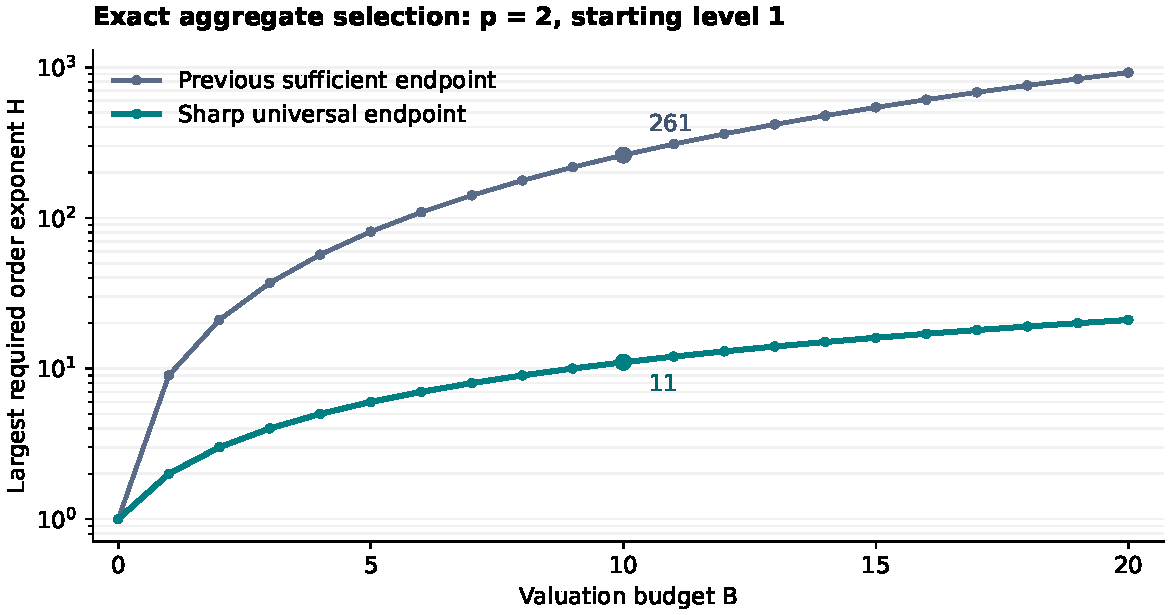
\includegraphics[width=.88\textwidth]{figures/order_bounds.pdf}
\caption{Endpoint comparison for \(p=2,h_0=1\). The vertical axis is logarithmic. The new endpoint is the exact universal threshold, while the predecessor supplied a conservative sufficient bound.}
\label{fig:bounds}
\end{figure}

At \(h_0=1\), the sharp answer simplifies to \(H_*=1+\lfloor B\rfloor\) for every prime. For an integer \(N\ge1\), the polynomial
\[
 g_N(T)=\prod_{h=1}^N\Phi_{p^h}(1+T)
       =\frac{(1+T)^{p^N}-1}{T}
\]
has \(G_\rho(g_N)=N\) for \(\rho\ge1/(p-1)\) and vanishes at every \(\zeta-1\) with \(\zeta\) a nontrivial \(p\)-power root of order at most \(p^N\). This gives an especially transparent witness that level \(N+1\) can really be necessary.

\subsection{Determinant and Fitting applications}
Let \(M_i(\mathbf T)\) be square matrices over bounded integral power series, and assume \(F_i=\det M_i\) is nonzero. If
\[
 \sum_iG_\rho(F_i)\le B,
\]
Corollary~\ref{cor:packets} gives a common torsion tuple at which all matrices are nonsingular and
\[
 \sum_i v(\det M_i(\mathbf z))\le\sum_iG_\rho(F_i).
 \tag{D}
\]
Thus the exact valuation of a product of denominator determinants can be kept within the original budget, with the optimal universal order ceiling.

If the data and the chosen torsion points lie in a finite extension \(L/\Qp\), Smith normal form gives
\[
 v_p(\det M_i(\mathbf z))
 =\frac{\operatorname{length}_{\Ocal_L}
             \operatorname{coker}M_i(\mathbf z)}
        {e(L/\Qp)}.
\]
Equation (D) therefore controls the sum of normalized finite colengths. Rectangular presentations can be treated by selecting nonzero minors, but the arithmetic presentation and its witness minors must first be supplied. The selection theorem does not construct them.

The source's denominator bookkeeping often aggregates losses, so this is a plausible place to use the stronger endpoint. Some source arguments require separate inequalities for each Selmer datum. The aggregate theorem alone is insufficient there, as the preceding counterexample proves. Replacing the source selector globally would require checking the actual objective at each call site.

\subsection{Several powers of the same parameter}
A standard product construction handles a finite list of powers, with a changed radius and budget. Suppose the integral series \(F_i\) have witness points of radius at least \(\rho\), with total valuation at most \(B\). For \(1\le j\le m\), consider
\[
 F_i\bigl((1+T_1)^j-1,\ldots,(1+T_s)^j-1\bigr).
\]
Each transformed series has a witness of coordinate valuations at least \(\rho/m\) and value equal to the original witness value. To see this, solve
\((1+y)^j=1+x\): its \(j\) roots are integral, and their valuations sum to \(v(x)\), so one has valuation at least \(v(x)/j\); if \(x=0\), take \(y=0\).

Choose \(h'_0\) with \(r_{h'_0}\le\rho/m\). Applying the sharp packet theorem with budget \(mB\) gives one tuple, of exponents at most
\[
 h'_0+\floor{p^{h'_0-1}mB},
\]
such that
\[
 \sum_{i,j}v\bigl(F_i(\zeta_1^j-1,\ldots,\zeta_s^j-1)\bigr)\le mB.
\]
The construction itself was already present in the prior exact report; the improvement here is the optimal underlying aggregate endpoint.

\subsection{Relation to existing local analysis}
The result should be compared with several established but different statements.

Bhargava's \(P\)-ordering framework organizes ultrametric interpolation and integer-valued polynomials \cite{bhargava}. The least-occupied residue branch in the proof is part of that general circle of ideas. Schefer studies quantitative \(p\)-adic Galois equidistribution of torsion points for logarithmic polynomial test functions \cite{schefer}. Those results concern averages and multiplicative independence, whereas this theorem solves an exact finite-grid worst-case problem.

Kriz--Nordentoft develop maximum-modulus principles in horizontal Iwasawa algebras and apply finite-order specialization to central-value nonvanishing \cite{kn}. This shows why a local selector is a useful arithmetic ingredient. It does not identify the present torsion-order ceiling with a global conductor ceiling: the relation between order, conductor, and admissible local behavior requires additional arithmetic information.

Serban's torsion-rigidity theorems include Lubin--Tate formal groups \cite{serban}. Our corollary concerns the sharp quantitative cost of finding one evaluation satisfying a fixed aggregate comparison; it does not strengthen the structural classification of torsion zero sets. We have established a strict improvement over the inspected ProveIt bound, but do not claim that the exact formula has never appeared elsewhere in the literature.

